\documentclass{howto}
\usepackage{distutils}
\usepackage{graphicx}
% $Id$

\title{What's New in MyHDL 0.3}
\release{0.3}
\author{Jan Decaluwe}
\authoraddress{\email{jan@jandecaluwe.com}}

\begin{document}
\maketitle
\tableofcontents


\section{VCD output for waveform viewing\label{section-wave}}

\ifpdf
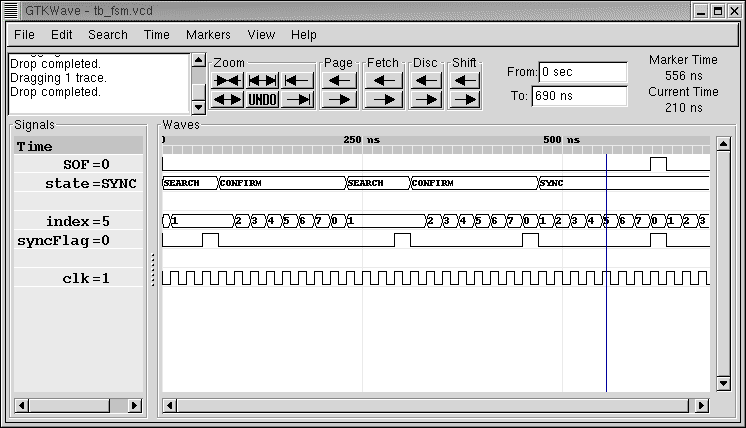
\includegraphics{tbfsm.png}
\fi

MyHDL now has support for waveform viewing. During simulation,
signal changes can be dumped in a VCD output file.
The VCD file can then be loaded in a waveform viewer tool.

The user interface of this feature consists of a single
function, \function{trace_sigs()}. It is used as follows. 
In MyHDL, instances are created by calling a function that
returns a sequence of generators. For example:

\begin{verbatim}
tb_fsm = testbench()
\end{verbatim}

To enable VCD tracing, the instance should be created as 
follows instead:

\begin{verbatim}
tb_fsm = trace_sigs(testbench)
\end{verbatim}

As a result, all signals in the hierarchy of the instance will be
traced in an output VCD file called \file{tb_fsm.vcd}. Note that the
argument of \function{trace_sigs()} consists of the uncalled
function. By calling the function under its control,
\function{trace_sigs()} gathers information about the hierarchy and
the signals to be traced.

In addition, \function{trace_sigs()} accepts an arbitrary number of
additional non-keyword and keyword arguments that will be passed
to the function call.




%======================================================================
\section{PEP 255: Simple Generators\label{section-generators}}

In Python 2.2, generators were added as an optional feature, to be
enabled by a \code{from __future__ import generators} directive.  In
2.3 generators no longer need to be specially enabled, and are now
always present; this means that \keyword{yield} is now always a
keyword.  The rest of this section is a copy of the description of
generators from the ``What's New in Python 2.2'' document; if you read
it back when Python 2.2 came out, you can skip the rest of this section.

You're doubtless familiar with how function calls work in Python or C.
When you call a function, it gets a private namespace where its local
variables are created.  When the function reaches a \keyword{return}
statement, the local variables are destroyed and the resulting value
is returned to the caller.  A later call to the same function will get
a fresh new set of local variables. But, what if the local variables
weren't thrown away on exiting a function?  What if you could later
resume the function where it left off?  This is what generators
provide; they can be thought of as resumable functions.

Here's the simplest example of a generator function:

\begin{verbatim}
def generate_ints(N):
    for i in range(N):
        yield i
\end{verbatim}

A new keyword, \keyword{yield}, was introduced for generators.  Any
function containing a \keyword{yield} statement is a generator
function; this is detected by Python's bytecode compiler which
compiles the function specially as a result.

When you call a generator function, it doesn't return a single value;
instead it returns a generator object that supports the iterator
protocol.  On executing the \keyword{yield} statement, the generator
outputs the value of \code{i}, similar to a \keyword{return}
statement.  The big difference between \keyword{yield} and a
\keyword{return} statement is that on reaching a \keyword{yield} the
generator's state of execution is suspended and local variables are
preserved.  On the next call to the generator's \code{.next()} method,
the function will resume executing immediately after the
\keyword{yield} statement.  (For complicated reasons, the
\keyword{yield} statement isn't allowed inside the \keyword{try} block
of a \keyword{try}...\keyword{finally} statement; read \pep{255} for a full
explanation of the interaction between \keyword{yield} and
exceptions.)

Here's a sample usage of the \function{generate_ints()} generator:

\begin{verbatim}
>>> gen = generate_ints(3)
>>> gen
<generator object at 0x8117f90>
>>> gen.next()
0
>>> gen.next()
1
>>> gen.next()
2
>>> gen.next()
Traceback (most recent call last):
  File "stdin", line 1, in ?
  File "stdin", line 2, in generate_ints
StopIteration
\end{verbatim}

You could equally write \code{for i in generate_ints(5)}, or
\code{a,b,c = generate_ints(3)}.

Inside a generator function, the \keyword{return} statement can only
be used without a value, and signals the end of the procession of
values; afterwards the generator cannot return any further values.
\keyword{return} with a value, such as \code{return 5}, is a syntax
error inside a generator function.  The end of the generator's results
can also be indicated by raising \exception{StopIteration} manually,
or by just letting the flow of execution fall off the bottom of the
function.

You could achieve the effect of generators manually by writing your
own class and storing all the local variables of the generator as
instance variables.  For example, returning a list of integers could
be done by setting \code{self.count} to 0, and having the
\method{next()} method increment \code{self.count} and return it.
However, for a moderately complicated generator, writing a
corresponding class would be much messier.
\file{Lib/test/test_generators.py} contains a number of more
interesting examples.  The simplest one implements an in-order
traversal of a tree using generators recursively.

\begin{verbatim}
# A recursive generator that generates Tree leaves in in-order.
def inorder(t):
    if t:
        for x in inorder(t.left):
            yield x
        yield t.label
        for x in inorder(t.right):
            yield x
\end{verbatim}

Two other examples in \file{Lib/test/test_generators.py} produce
solutions for the N-Queens problem (placing $N$ queens on an $NxN$
chess board so that no queen threatens another) and the Knight's Tour
(a route that takes a knight to every square of an $NxN$ chessboard
without visiting any square twice).

The idea of generators comes from other programming languages,
especially Icon (\url{http://www.cs.arizona.edu/icon/}), where the
idea of generators is central.  In Icon, every
expression and function call behaves like a generator.  One example
from ``An Overview of the Icon Programming Language'' at
\url{http://www.cs.arizona.edu/icon/docs/ipd266.htm} gives an idea of
what this looks like:

\begin{verbatim}
sentence := "Store it in the neighboring harbor"
if (i := find("or", sentence)) > 5 then write(i)
\end{verbatim}

In Icon the \function{find()} function returns the indexes at which the
substring ``or'' is found: 3, 23, 33.  In the \keyword{if} statement,
\code{i} is first assigned a value of 3, but 3 is less than 5, so the
comparison fails, and Icon retries it with the second value of 23.  23
is greater than 5, so the comparison now succeeds, and the code prints
the value 23 to the screen.

Python doesn't go nearly as far as Icon in adopting generators as a
central concept.  Generators are considered part of the core
Python language, but learning or using them isn't compulsory; if they
don't solve any problems that you have, feel free to ignore them.
One novel feature of Python's interface as compared to
Icon's is that a generator's state is represented as a concrete object
(the iterator) that can be passed around to other functions or stored
in a data structure.

\begin{seealso}

\seepep{255}{Simple Generators}{Written by Neil Schemenauer, Tim
Peters, Magnus Lie Hetland.  Implemented mostly by Neil Schemenauer
and Tim Peters, with other fixes from the Python Labs crew.}

\end{seealso}


%======================================================================
\section{Other Language Changes}

Here are all of the changes that Python 2.3 makes to the core Python
language.

\begin{itemize}
\item The \keyword{yield} statement is now always a keyword, as
described in section~\ref{section-generators} of this document.

\item A new built-in function \function{enumerate()}
was added, as described in section~\ref{section-enumerate} of this
document.

\item Two new constants, \constant{True} and \constant{False} were
added along with the built-in \class{bool} type, as described in
section~\ref{section-bool} of this document.

\item The \function{int()} type constructor will now return a long
integer instead of raising an \exception{OverflowError} when a string
or floating-point number is too large to fit into an integer.  This
can lead to the paradoxical result that
\code{isinstance(int(\var{expression}), int)} is false, but that seems
unlikely to cause problems in practice.

\item Built-in types now support the extended slicing syntax,
as described in section~\ref{section-slices} of this document.

\item Dictionaries have a new method, \method{pop(\var{key})}, that
returns the value corresponding to \var{key} and removes that
key/value pair from the dictionary.  \method{pop()} will raise a
\exception{KeyError} if the requested key isn't present in the
dictionary:

\begin{verbatim}
>>> d = {1:2}
>>> d
{1: 2}
>>> d.pop(4)
Traceback (most recent call last):
  File "stdin", line 1, in ?
KeyError: 4
>>> d.pop(1)
2
>>> d.pop(1)
Traceback (most recent call last):
  File "stdin", line 1, in ?
KeyError: 'pop(): dictionary is empty'
>>> d
{}
>>>
\end{verbatim}

There's also a new class method, 
\method{dict.fromkeys(\var{iterable}, \var{value})}, that 
creates a dictionary with keys taken from the supplied iterator
\var{iterable} and all values set to \var{value}, defaulting to
\code{None}.  

(Patches contributed by Raymond Hettinger.)

Also, the \function{dict()} constructor now accepts keyword arguments to
simplify creating small dictionaries:

\begin{verbatim}
>>> dict(red=1, blue=2, green=3, black=4)
{'blue': 2, 'black': 4, 'green': 3, 'red': 1}    
\end{verbatim}

(Contributed by Just van~Rossum.)       

\item The \keyword{assert} statement no longer checks the \code{__debug__}
flag, so you can no longer disable assertions by assigning to \code{__debug__}.
Running Python with the \programopt{-O} switch will still generate
code that doesn't execute any assertions.

\item Most type objects are now callable, so you can use them
to create new objects such as functions, classes, and modules.  (This
means that the \module{new} module can be deprecated in a future
Python version, because you can now use the type objects available in
the \module{types} module.)
% XXX should new.py use PendingDeprecationWarning?
For example, you can create a new module object with the following code:

\begin{verbatim}
>>> import types
>>> m = types.ModuleType('abc','docstring')
>>> m
<module 'abc' (built-in)>
>>> m.__doc__
'docstring'
\end{verbatim}

\item
A new warning, \exception{PendingDeprecationWarning} was added to
indicate features which are in the process of being
deprecated.  The warning will \emph{not} be printed by default.  To
check for use of features that will be deprecated in the future,
supply \programopt{-Walways::PendingDeprecationWarning::} on the
command line or use \function{warnings.filterwarnings()}.

\item The process of deprecating string-based exceptions, as
in \code{raise "Error occurred"}, has begun.  Raising a string will
now trigger \exception{PendingDeprecationWarning}.

\item Using \code{None} as a variable name will now result in a
\exception{SyntaxWarning} warning.  In a future version of Python,
\code{None} may finally become a keyword.

\item The method resolution order used by new-style classes has
changed, though you'll only notice the difference if you have a really
complicated inheritance hierarchy.  (Classic classes are unaffected by
this change.)  Python 2.2 originally used a topological sort of a
class's ancestors, but 2.3 now uses the C3 algorithm as described in
the paper \ulink{``A Monotonic Superclass Linearization for
Dylan''}{http://www.webcom.com/haahr/dylan/linearization-oopsla96.html}.
To understand the motivation for this change, 
read Michele Simionato's article 
\ulink{``Python 2.3 Method Resolution Order''}
      {http://www.python.org/2.3/mro.html}, or
read the thread on python-dev starting with the message at
\url{http://mail.python.org/pipermail/python-dev/2002-October/029035.html}.
Samuele Pedroni first pointed out the problem and also implemented the
fix by coding the C3 algorithm.

\item Python runs multithreaded programs by switching between threads
after executing N bytecodes.  The default value for N has been
increased from 10 to 100 bytecodes, speeding up single-threaded
applications by reducing the switching overhead.  Some multithreaded
applications may suffer slower response time, but that's easily fixed
by setting the limit back to a lower number using
\function{sys.setcheckinterval(\var{N})}.

\item One minor but far-reaching change is that the names of extension
types defined by the modules included with Python now contain the
module and a \character{.} in front of the type name.  For example, in
Python 2.2, if you created a socket and printed its
\member{__class__}, you'd get this output:

\begin{verbatim}
>>> s = socket.socket()
>>> s.__class__
<type 'socket'>
\end{verbatim}

In 2.3, you get this:
\begin{verbatim}
>>> s.__class__
<type '_socket.socket'>
\end{verbatim}

\item One of the noted incompatibilities between old- and new-style
  classes has been removed: you can now assign to the
  \member{__name__} and \member{__bases__} attributes of new-style
  classes.  There are some restrictions on what can be assigned to
  \member{__bases__} along the lines of those relating to assigning to
  an instance's \member{__class__} attribute.

\end{itemize}




\end{document}
